\chapter{Contribution}
\label{chap:contrib}
\textit{\initial{F}rom the experiments conducted in Chapter 2, we identified a set of problems and designed our solution based on the observations made. This chapter presents our architecture and describes the different modules of which it is constituted. The plan of this chapter is as follows:
}

\minitoc

\newpage
In the previous chapter, we demonstrate the consequences of a non-intelligent allocation of resources to the dom0. To solve this problem, we propose an architecture of dom0 which will respect the following three principles:

\begin{enumerate}
    \item the dom0 must have exactly the amount of resources it needs at every moment,
    \item the processes that work on behalf of virtual machines must use the resources of these virtual machines and 
    \item these processes must be executed as close as possible to the virtual machines for which they work.
\end{enumerate}

We propose an architecture in which dom0 is a kind of multi-kernel \citep{multikernel}, as shown in Figure \ref{fig:multidom0}. It is organized in containers of two types: a \textbf{main container} and \textbf{secondary containers}. The following sections describe the contents of each container.

\begin{figure}[!h]
    \centering
    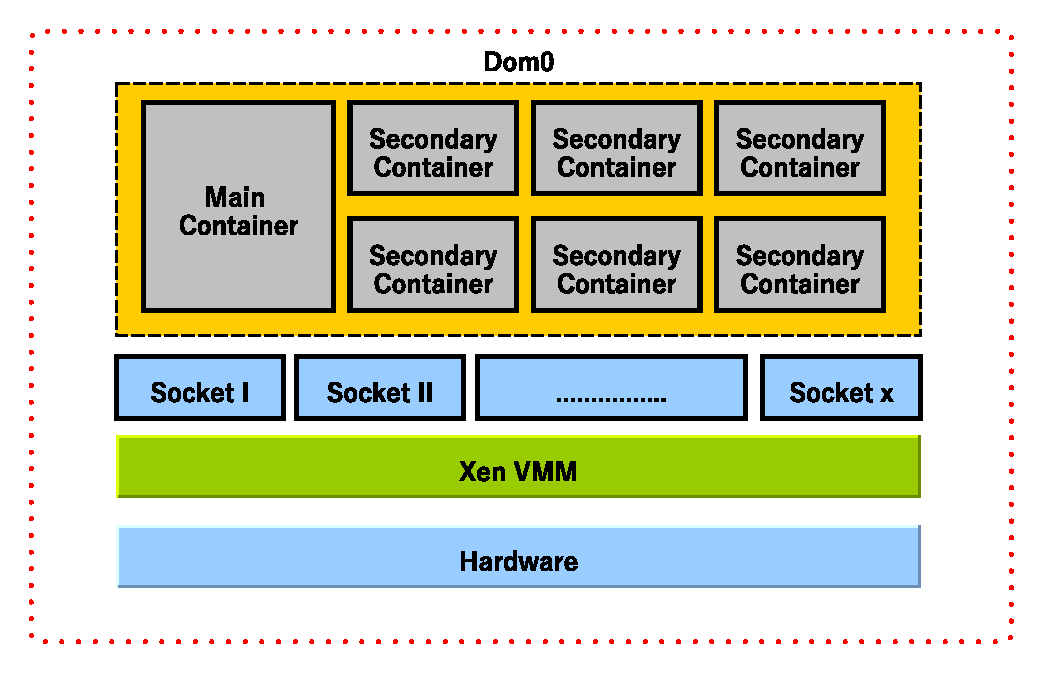
\includegraphics[width=\linewidth]{fig04/multidom0.pdf}
    \caption{Our dom0 design}
    \label{fig:multidom0}
\end{figure}

\newpage 
\section{Container composition}
We have organized the processes of dom0 into four groups, see table \ref{table:group_dom0}, $(T_o)$ the basic processes of a Linux system, $(T_1)$ management processes for the \glspl{dc}, $(T_2)$ the virtual machine administration processes, and $(T_3)$ the management processes of \acrshort{io}. The tasks of $T_o, T_2 $ and part of $T_2$ (excluding the tasks of shutdown and migration of virtual machines) constitute the main container. These are processes whose resource consumption is almost constant (section 3.2). As for the secondary container, it consists of virtual machine migration and shutdown processes and all processes of $T_3$. The resource consumption of these processes depends on the target virtual machines. The number of secondary containers corresponds to the number of sockets dedicated to Domus (section 3.3).

The process creation task has been modified to take this classification into account. Each processor is identified by its category and assigned in the right container. The same is true for \acrshort{vcpu}s containers. A \acrshort{vcpu} is of either of type \textbf{main} or \textbf{secondary} depending on its container. 

\begin{table}[!h]
    \centering 
     \caption{Dom0 processes organization}
    \begin{tabular}{cc}
        \toprule
        \textbf{Group Designation} & \textbf{Processes included} \\
             \myrowcolour
        $T_o$ & Basic processes of a Linux system \\
        $T_1$ & \gls{dc} management processes\\
             \myrowcolour
        $T_2$ & VM administration processes \\
        $T_3$ & \acrshort{io} management processes \\
        \bottomrule
    \end{tabular}
    \label{table:group_dom0}
\end{table}

VM: Virtual Machine.


\section{Resource allocation to the main container}
A number of resources consumed by the main container processes must be supported by the provider, unlike the secondary container processes. Moreover, these resources have no need to be close to the Domus. On the contrary, they would harm each other. The number of resources consumed by the main container is constant. Figure \ref{fig:conNo} shows the consumption of these processes as part of a \glspl{dc} handled by OpenStack (minimalist architecture as on Figure \ref{fig:miniO}). We see that regardless of the number of virtual machines on the server, these processes (essentially the \textbf{nova-compute}) consume the same amount of memory and \acrshort{cpu}. Note also that this consumption does not depend on the number of servers in the \glspl{dc} but on the complexity of the OpenStack architecture set up. In this OpenStack standard configuration, we estimated that the allocation of 2 processes and 2\acrshort{gb} of memory to the main container is sufficient. Thus, for the allocation of the resources of the main container, we propose a static allocation estimated by the provider. Table \ref{table:confDc} gives several configurations for the minimalistic architecture of OpenStack, Eucalyptus, and OpenNebula, three reputed cloud \glspl{dc} frameworks.


\begin{table}[!h]
    \centering
        \caption{\gls{dc} minimalistic architecture consumption}

    \begin{tabular}{ccccccccccc}
    \toprule
    \multirow{3}*{DC Tool} & \multicolumn{10}{c}{\textbf{Number of Virutal machines}} \\
    \myrowcolour
    & \multicolumn{2}{c}{\textbf{10}} & \multicolumn{2}{c}{\textbf{20}} & \multicolumn{2}{c}{\textbf{30}} & \multicolumn{2}{c}{\textbf{40}} & \multicolumn{2}{c}{\textbf{50}} \\
    & VCPU & Mem & VCPU & Mem & VCPU & Mem & VCPU & Mem  & VCPU & Mem \\
    \myrowcolour
    \textbf{Euc} & 1 & 1.5 & 1 & 1.5 & 1 & 1.5 & 1 & 1.5 & 1 & 1.5 \\
    \textbf{OpN} & 2 & 1.85 & 2 & 1.85 & 2 & 1.85 & 2 & 1.85 & 2 & 1.85 \\
    \myrowcolour
    \textbf{OpS} & 2 & 2 & 2 & 2 & 2 & 2 & 2 & 2 & 2 & 2 \\
    \bottomrule 
    \end{tabular}
    \label{table:confDc}
\end{table}
\begin{itemize}
\item Euc = Eucalyptus, OpN = OpenNebula, OpS = OpenStack, Mem = Memory.
\item VCPU stands for the number of VCPU required. 
\item All the memory values are in \acrshort{gb}.
\end{itemize}
%%%%%%%%%%%%%%%%%%%%%%%%%%%%%%%%%%
\begin{figure}[!h]
\begin{minipage}[b]{.5\linewidth}
\centering 
  \begin{tikzpicture}
  \begin{axis}[legend style={at={(0.5,-0.1)},anchor=north},
  title = {Nova Compute Memory Consumption},
  ymin = 0,
  legend entries = {Memory (\acrshort{gb})}]
  \addplot table {chapters/chapter04/data/expe2.dat};
  \end{axis}
  \end{tikzpicture}
\subcaption{Memory Consumption}
\end{minipage}
\begin{minipage}[b]{.5\linewidth}
\centering 
  \begin{tikzpicture}
  \begin{axis}[legend style={at={(0.5,-0.1)},anchor=north},
  title = {Nova Compute VCPU load},
    ymin = 0,
  legend entries = {2 VCPU load (\%) }]
  \addplot table {chapters/chapter04/data/expe1.dat};
  \end{axis}
  \end{tikzpicture}
\subcaption{VCPU load}
\end{minipage}
\caption{OpenStack Minimalistic set-up consumption}
\label{fig:conNo}
\end{figure}
%%%%%%%%%%%%%%%%%%%%%%%%%%%%%

\begin{figure}[!h]
    \centering
    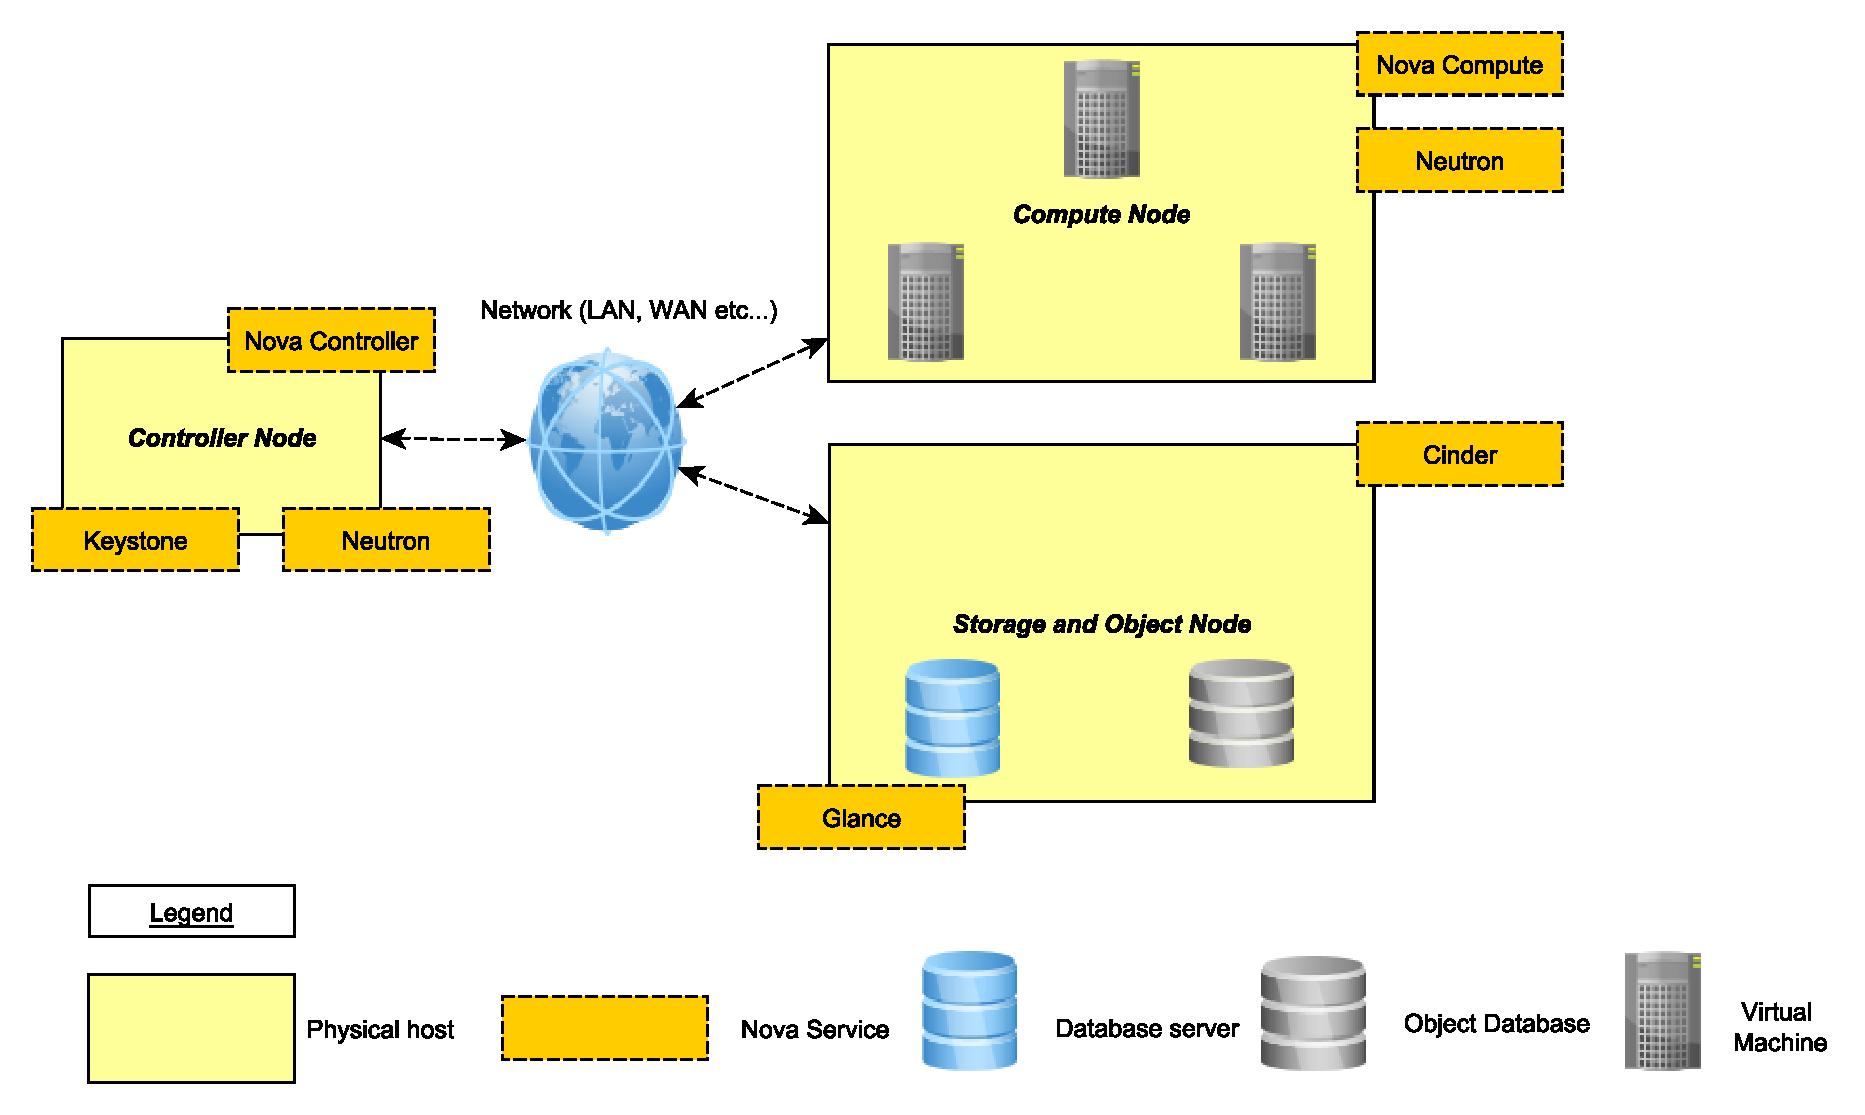
\includegraphics[width=\linewidth]{fig04/minimalArchiOpentStack.pdf}
    \caption{Minimal OpenStack architecture set-up}
    \label{fig:miniO}
\end{figure}

\section{Resource allocation to secondary containers}
Among the tasks that are in a secondary container, we have the tasks of virtual machine administrations and \acrshort{io} management tasks. The first ones are created only when needed while the seconds are created when the server starts. The allocation of resources to these tasks must be gently done because their activities depend on the domains and their localities can affect the performance of these domains. To do this, we associate a secondary container per \acrshort{numa} socket so that a virtual machine that runs on the socket $ x $ is managed by the secondary container of this socket. The resources of a secondary container are restricted to its socket. In addition, the resources consumed by the secondary containers are taken from the resource quota of the domU. The following sections introduce \textbf{our scheduling algorithms} for these tasks.


\subsection{Memory allocation}
After the server starts (no domU), each secondary container contains only the back-end management processes of \acrshort{io} that do not run. The amount of memory used by this back-end is negligible ($44\acrshort{kb}$ in the case of Xen). This amount of memory is assumed by the provider, as well as the memory that will be used by the processes of migration and shutdown of virtual machines. Thus the initial size of a secondary container is $75\acrshort{mb}$, which is negligible. The size of the memory will be adapted according to the activity of the domU. Let $M$ be the amount of memory requested by a domU that must be started. Let n be the number of sockets on which the domU will be executed. Thus the amount of memory that will actually be given to the VM at startup will be $\mathbf{M-n\times\epsilon}$, $\epsilon$ will be the initial contribution of the domU in each secondary container. $\epsilon$ corresponds the amount of memory used by dom0. The possible values of $\epsilon$ can be calculated beforehand by studying all the types of file system executed by the cloud (on Amazon, for example, we know all types of instances in advance). Once the virtual machine is started, it can be called up (ballooning) according to the intensity of its activities \acrshort{io}. The claim policy is made in increments of intensity and the memory is always requested in advance for each level passed. Note that when the intensity decreases, the virtual machine will be given back the memory.


\begin{algorithm}
\caption{Memory Allocation for the secondary container in charge of the virtual machine \textbf{VM} using the defined parameter $\mathbf{\epsilon}$}
\begin{algorithmic}[1]
\Procedure{SecMemAlloc}{VM, $\epsilon$}
\State $\textit{M} \gets \text{MemoryRequested (VM)}$ \Comment{Get the VM memory size at creation}
\State $n \gets \text{SocketNumber (VM)}$ 
\BState \emph{initialization}:
\State $secMem = M - (n\times\epsilon)$
\BState \emph{loop}:
\If {VMIOIncreasing(VM)} \Comment{If the \acrshort{io} intensity of VM is increasing}
\State $reserve \gets $ BalloonReserve (VM) \Comment{Increase secondary container's memory}
\State $secMem \gets secMem + reserve $ . \Comment{by removing from VM's memory}
\State \textbf{goto} \emph{loop}.
\Else 
    \If {VMIODecreasing (VM)}\Comment{If the \acrshort{io} intensity of VM is decreasing}
        \State GiveBackMem (VM,$secMem$)
    \EndIf
\State \textbf{goto} \emph{loop}.
\EndIf
\EndProcedure
\end{algorithmic}
\end{algorithm}

\subsection{Processor allocation}
At server startup, dom0 is created with as many \acrshort{vcpu}s as there are processors on the server. \acrshort{vcpu}s allocated to the main container (tagged main \acrshort{vcpu}) are pinned to their processors and are never rescheduled. Here we are interested in other \acrshort{vcpu} (tagged secondary \acrshort{vcpu}), used by secondary containers. At server startup, each of these \acrshort{vcpu}s are pinned to a processor (except those used by the \acrshort{vcpu} tagged main) but is not scheduled. They will be used whenever necessary, according to the algorithm Figure \ref{fig:algo}.

\paragraph{domU shutdown and migration operations.} When one of these operations is requested, the associated process is created and assigned to the secondary container of the socket on which the greatest amount of memory of the target virtual machine is located. Then, the \acrshort{vcpu} that will execute the operation is the one that has been pinned to the processor currently used by the target \acrshort{vcpu}. In this way, the processes are executed next to the memory of the target virtual machines, which accelerates their execution (these processes work mainly on the memory). Using one of the processors of the virtual machine can be seen as a problem in the migration, slowing down the execution of the virtual machine. This slowdown accelerates the migration operation because it reduces the frequency of modification of the memory pages by the virtual machine. This allows you to quickly migrate the VM \citep{livemigration,livemigration2}. The evaluations confirm this.

\begin{algorithm}
\caption{Task Scheduling for a secondary container in charge of virtual machine \textbf{VM}}
\begin{algorithmic}[1]
\Procedure{SecMemAlloc}{VM}
\State $\textit{secCon} \gets \text{GreatestMemSocket (VM)}$ 
\State $vcpu \gets \text{pinnedVCPU (VM,secCon)}$ 
\State $\text{Schedule(secCon,vcpu)}$ 
\EndProcedure
\end{algorithmic}
\end{algorithm}

\paragraph{\acrshort{io} management operations.}These operations are of two types: the operations initiated by the domU and the operations not initiated by the domU. In the first type, we have read and write disk operations, and packet sending operations on the network. In the second type, we have the receiption of packets. Our policy of allocating processors to these processes in the case of operations initiated by the VM consists in scheduling them on one of the \acrshort{vcpu}s of the secondary container and this \acrshort{vcpu} will in turn scheduler on the processor which was used by the \acrshort{vcpu} of the virtual machine having initiated the operation (in the case of the tasks initiated by the virtual machine). For external operations, the processes of the secondary container responsible for processing the operation are scheduled on one of the processes used by the target VM. \acrshort{vcpu}s will be chosen fairly. The implementation of this policy in Xen is quite fast. For operations initiated by the VM, it is easy to know the \acrshort{vcpu} that initiated the operation. This is the \acrshort{vcpu} that generates the virtual interrupt to signal to the back-end the presence of an operation in the ring buffer (in chapter 1). For external operations, it is sufficient to count the participation of each \acrshort{vcpu} of the secondary container and to choose the one that contributed the least. This is the processor, which will be responsible for processing the operation in question.  It is another \acrshort{vcpu} of the virtual machine that will receive the virtual interrupt saying that a packet is present.

\section{Our approach advantages}

Th new dom0 design we came up with, present a number of advantages which are : 

\begin{itemize}
    \item \textbf{Predictability}: The performance of virtual machines will not be disturbed by the activities of neighboring guests, so the yield should be what is expected.
    \item \textbf{Locality}: Each time the dom0 will have to work on behalf of a virtual machine, its resources will be co-located with those of the virtual machine target, thus preventing remote accesses.
    \item \textbf{Accounting/Billing}: Each virtual machine will consume a number of resources requests at startup since the dom0 uses the virtual machine resources to realize their work.
    
    \item \textbf{Scalability}: This approach allows the dom0 to be scalable by distributing its resources over the entire hardware architecture.
\end{itemize}

\begin{figure}[!h]
    \centering
    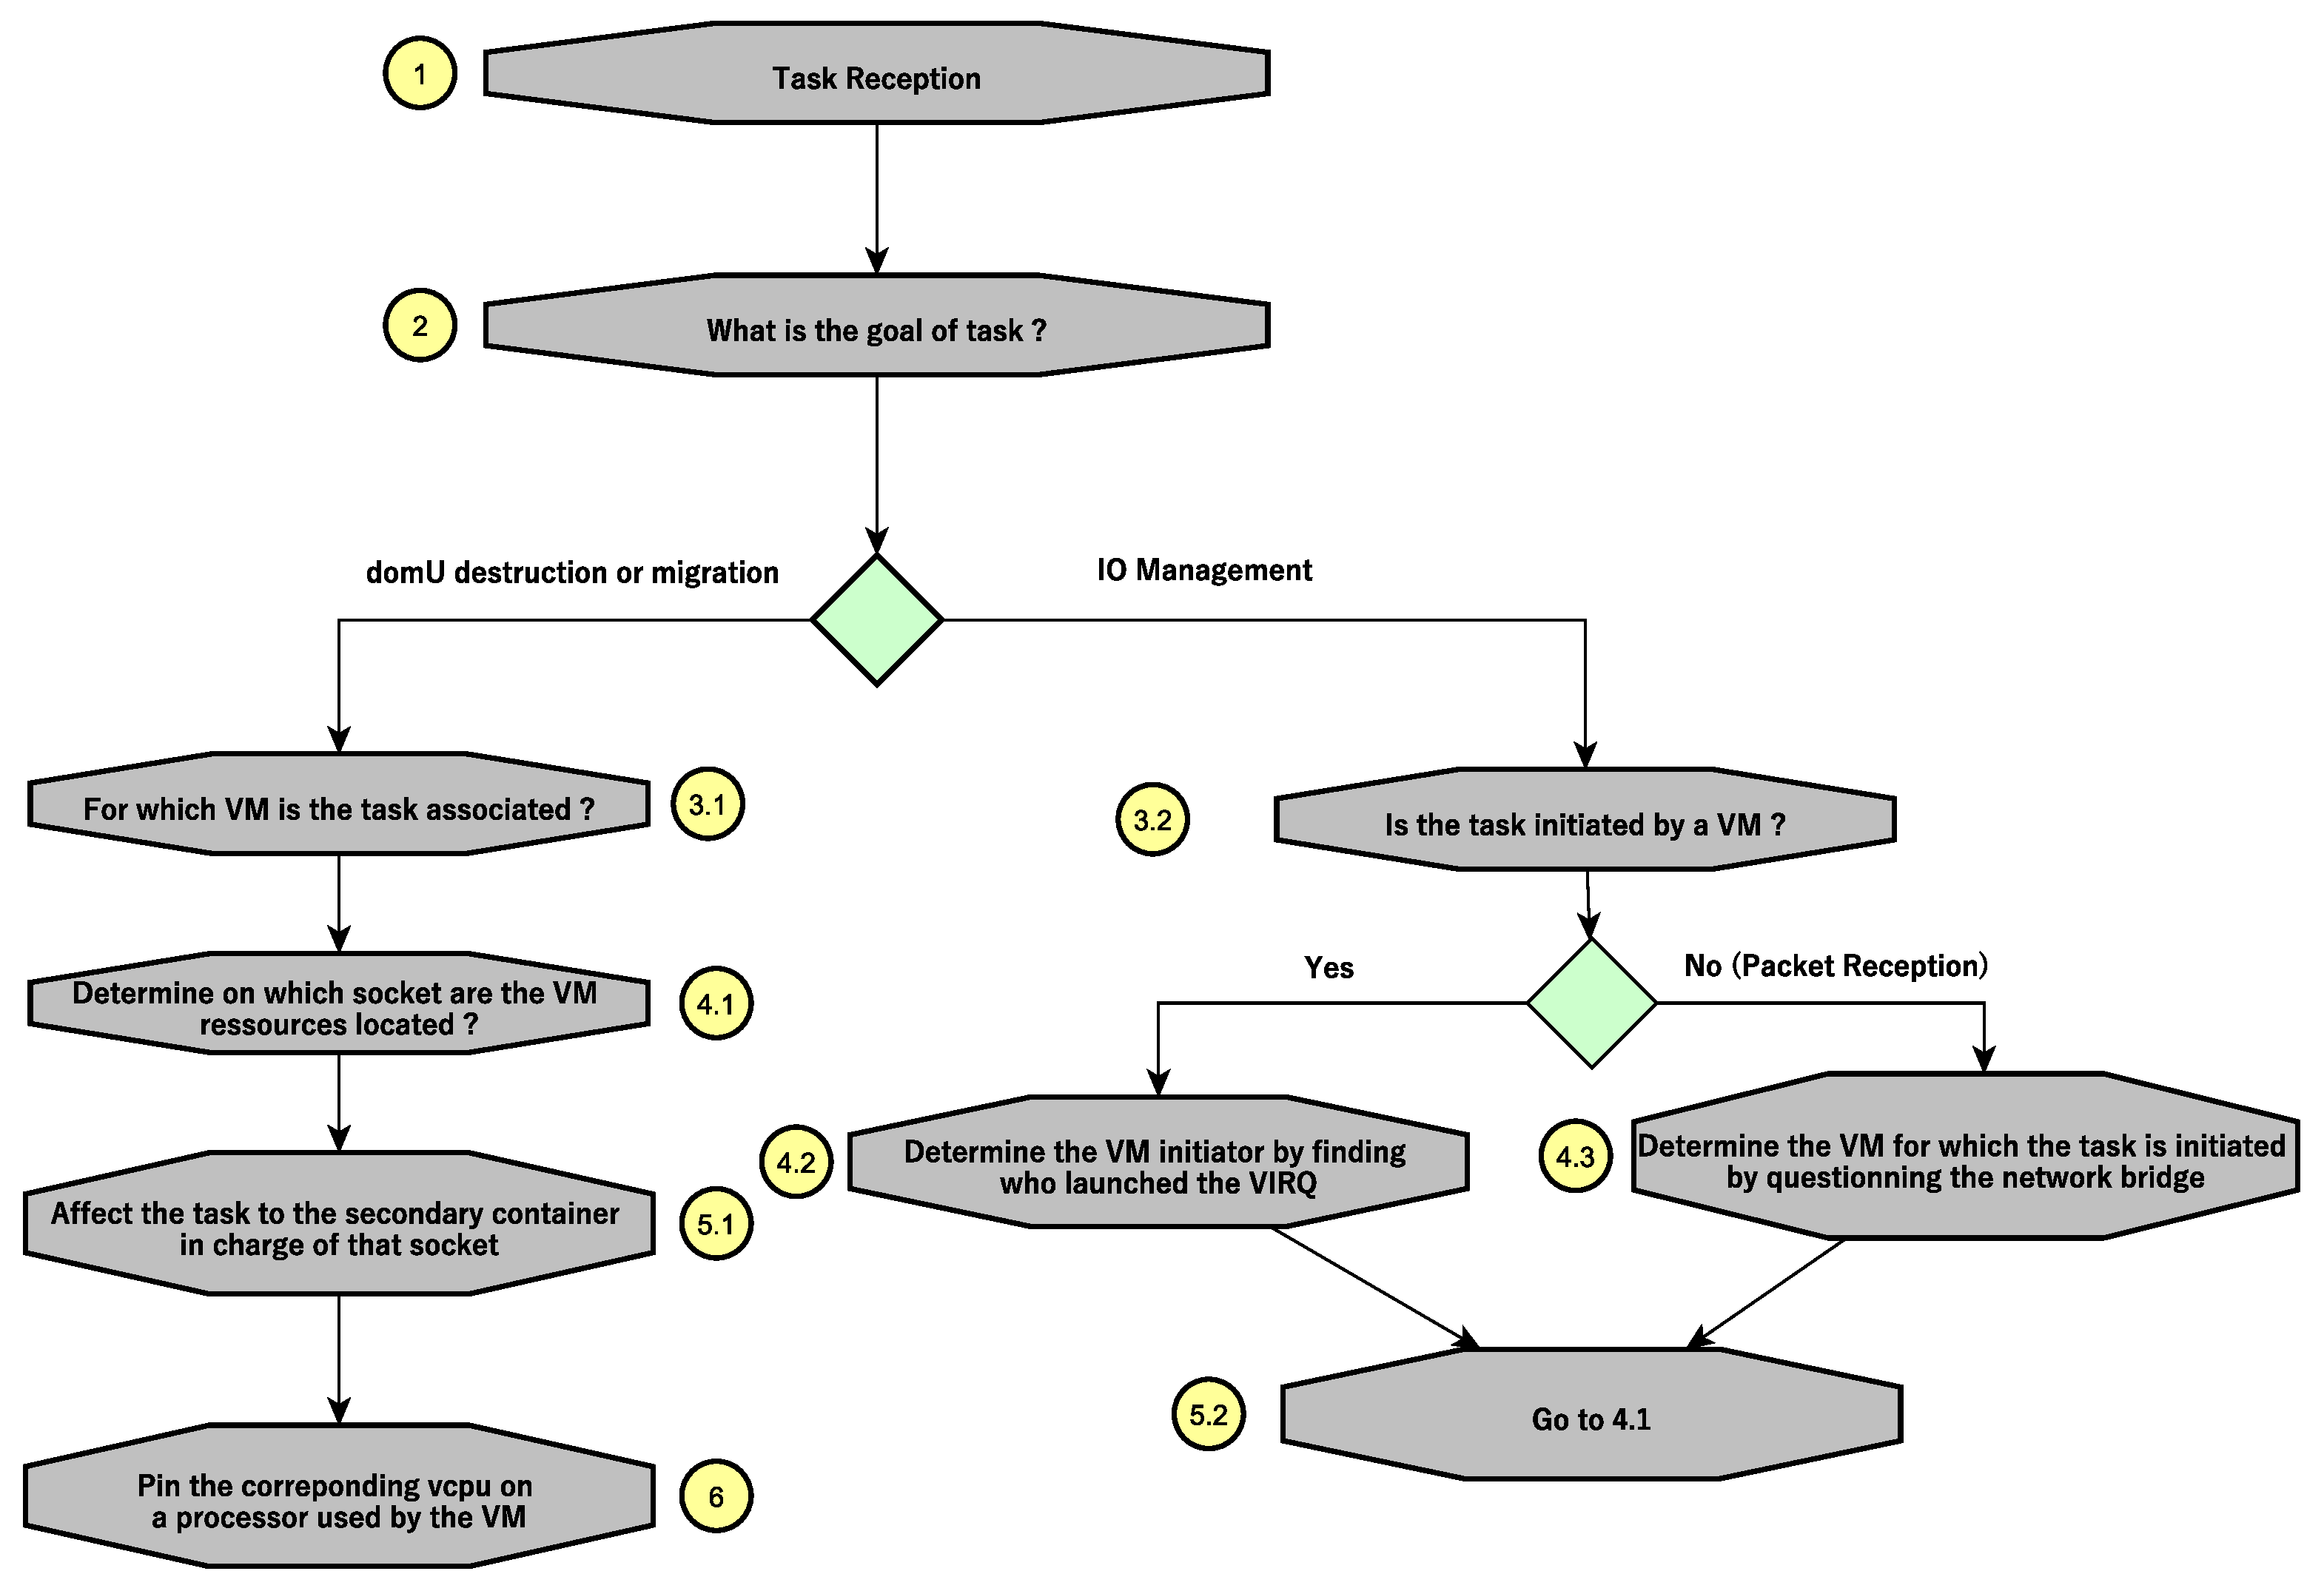
\includegraphics[scale=0.35]{fig04/algoSecondGroupSchedulingDom0.pdf}
    \caption{Scheduling Algorithm for secondary dom0 tasks}
    \label{fig:algo}
\end{figure}
\vspace{-1cm}
